\documentclass[12pt,letterpaper]{book}
\usepackage[width=6.5in, height=9.0in, top=1.25in, papersize={8.5in,11in}]{geometry}
\usepackage[utf8]{inputenc}	%encoding para el teclado espa–ol
%\usepackage[latin1]{inputenc}
%\usepackage[spanish]{babel}		%Para cambiar figure por figura y demas automatizaciones
\usepackage[pdftex]{graphicx}
\usepackage{amsmath}
\usepackage{amssymb}
%\usepackage{tipa}
%\usepackage{txfonts}
\usepackage{textcomp}
%\usepackage{amsthm}
%\usepackage{array}
%\usepackage{xy}
\usepackage[font={footnotesize,it},width=13cm]{caption}

\usepackage{fancyhdr}
\pagestyle{fancy}
\renewcommand{\chaptermark}[1]{\markboth{#1}{}}
\renewcommand{\sectionmark}[1]{\markright{\thesection\ #1}}
\fancyhf{}
\fancyhead[LE,RO]{\bfseries\thepage}
\fancyhead[LO]{\bfseries\rightmark}
\fancyhead[RE]{\bfseries\leftmark}
\renewcommand{\headrulewidth}{0.5pt}
\renewcommand{\footrulewidth}{0pt}
\addtolength{\headheight}{0.5pt}
\setlength{\footskip}{0in}
\renewcommand{\footruleskip}{0pt}
\fancypagestyle{plain}{%
\fancyhead{}
\renewcommand{\headrulewidth}{0pt}
}

\usepackage{listings} % Required for inserting code snippets
\usepackage[usenames,dvipsnames]{color} % Required for specifying custom colors and referring to colors by name

\definecolor{gray97}{gray}{.97}
\definecolor{gray75}{gray}{.75}
\definecolor{gray45}{gray}{.45}

\lstset{ frame=Ltb,
framerule=0pt,
aboveskip=0.5cm,
framextopmargin=3pt,
framexbottommargin=3pt,
framexleftmargin=0.4cm,
framesep=0pt,
rulesep=.4pt,
backgroundcolor=\color{gray97},
rulesepcolor=\color{black},
%
stringstyle=\ttfamily ,
showstringspaces = false,
basicstyle=\small\ttfamily ,
commentstyle=\color{gray45},
keywordstyle=\bfseries,
%
numbers=left,
numbersep=15pt,
numberstyle=\tiny,
numberfirstline = false,
breaklines=true,
}

% minimizar fragmentado de listados
\lstnewenvironment{listing}[1][]
{\lstset{#1}\pagebreak[0]}{\pagebreak[0]}
\lstdefinestyle{consola}
{basicstyle=\scriptsize\bf\ttfamily,
backgroundcolor=\color{gray75},
}
\lstdefinestyle{C}
{language=C,
}

\renewcommand{\chaptername}{Capítulo}
\renewcommand{\contentsname}{Contenido}

%
%\parindent 0in
\parskip 0.05in
%
\begin{document}
\frontmatter
%
\chapter*{\Huge \center Programación por memoria compartida }
\thispagestyle{empty}
{\hspace{2in} 
\includegraphics{../imagenes/logo_lufac.png} }
%\section*{\huge \center José María Zamora Fuentes}
%\section*{\huge \center Manuel Almaraz }
\newpage
\subsection*{\center \normalsize Traducción por:}
\subsection*{\center \normalsize José María Zamora Fuentes}
\subsection*{\center \normalsize Manuel Alejandro Almaraz Benítez }
\subsection*{\center \normalsize Tomado de:}
\subsection*{\center \normalsize Parallel Programming in C with MPI and OpenMP}
\subsection*{\center \normalsize Michael J. Quinn}
\subsection*{\center \normalsize McGraw-Hill Education Group \copyright 2003 }
\subsection*{\center \normalsize All rights reserved.}
\subsection*{\center \normalsize ISBN 0071232656}
%
%\chapter*{\center \normalsize To my Son}
%
\tableofcontents
%
\mainmatter
%
\chapter{OpenMP}
\newpage
\section{El modelo de memoria compartida}
El modelo de memoria compartida se muestra en la figura \ref{fig:shared_mem} %es una abstraccion de él modelo genérico mostrado en la FIGURA X. 
El hardware subyacente a este modelo es entendido como una colección de procesadores cada cual con acceso a la misma memoria compartida. Debido a que cada procesador puede acceder a las mismas localidades de memoria, estos pueden interactuar y ser sincronciados  por medio de variables compartidas.

\begin{figure}[ht]
\begin{center}
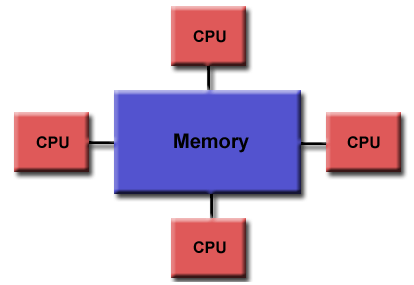
\includegraphics[width=5cm]{../imagenes/shared_mem.png} 
\end{center}
\caption{Modelo de memoria compartida}
\label{fig:shared_mem}
\end{figure}

La perspectiva estandar del paralelismo en un programa que usa memoria compartida es el paralelismo \textbf{fork/join}. Cuando el programa comienza la ejecución, sólo existe activo un hilo, llamado \textbf{hilo maestro} (Figura \ref{fig:fork_join}). El hilo maestro ejecuta las porciones secuenciales del algoritmo. En algún punto serán requeridas operaciones paralelas, en ese momento el hilo maestro se bifurca (\textbf{fork}), es decir, crea hilos adicionales. El hilo maestro y los hilos creados trabajan concurrentemente a través de la sección paralela. Al final del código paralelo, los hilos creados \textit{mueren} o son suspendidos, y el flujo de control regresa al hilo maestro, esto es conocido como unión(\textbf{join}).

La diferencia clave, entre el modelo de memoria compartida (MMC) y el modelo de paso de mensajes (MPM) es que en MPM todos los procesos típicamente permenecen activos durante la ejecución de todo el programa, mientras en el modelo de memoria compartida sólo hay un hilo activo al inicio del programa y al final, los hilos se crean y mueren dinámicamente.

Uno puede ver un programa secuencial como un caso especial de un programa paralelo por memoria compartida: simplemente es un programa que no realiza ningún \textbf{fork}, ni un \textbf{join}. De ahí que podemos decir, que el modelo de memoria compartida soporta la \textbf{paralelización incremental}. Es decir, transformar un programa secuencial en un programa paralelo puede ser realizado por bloques de código ó en etapas.

La paralelizacion incremental es una de las grandes ventajas del MMC sobre el MMP. Esto permite seccionar la ejecución de un programa secuencial, ergo, ordenar el programa en bloques de acuerdo a cuanto consume de recursos cada uno. Paralelizar sólo los bloques críticos en cuanto a consumo de CPU, y dejar los demás bloques intactos, puede ahorrar demasiado tiempo de codificación.

Consideremos, por el contrario, los programas de paso de mensajes. Ellos no tienen variables de retención de memoria compartida y los procesos paralelos son activos durante la ejecución del programa. La transformación de un programa secuencial en un programa paralelo no es incremental en absoluto (el abismo se debe cruzar con un gran salto, en lugar de muchos pequeños pasos).

\begin{figure}
\begin{center}
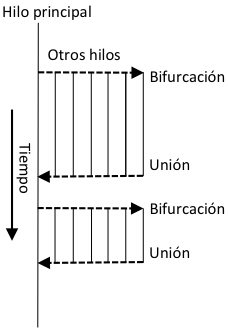
\includegraphics[width=4cm]{../imagenes/fork_join.png} 
\end{center}
\caption{Modelo de memoria compartida}
\label{fig:fork_join}
\end{figure}


%%%%%%%%%%%%%%%%%%%%%%%%%%%%%%%%%%%%%%%%%
\section{Loops paralelos usando for}
Operaciones intrínsecamente paralelas se expresan a menudo en los programas de C como bucles tipo \textbf{for}. OpenMP hace que sea fácil indicar cuando las iteraciones del ciclo pueden ser ejecutadas en paralelo. Por ejemplo, considere el siguiente ciclo, que representa una gran parte del tiempo de ejecución en una implementación:

\begin{lstlisting}[style=C]
for (i=first; i<size; i+=prime) marked[i] = i
\end{lstlisting}

Claramente no hay una dependencia de datos entre una iteración del ciclo y otra sentencia. ¿Cómo se puede convertir este ciclo secuencial en un ciclo paralelo?. En OpenMP simplemente indicamos al compilador que las iteraciones de un bucle pueden ser ejecutadas en paralelo, el compilador se encarga de generar el código que bifurca y une los hilos, además de que controlará la asignación de las iteraciones a los hilos de manera automática (\textbf{schedules}).

\section{\textit{parallel for} \textbf{Pragma}}
Una directiva para el compilador en C o C++ es llamada \textbf{pragma}. La palabra \textit{pragma} es la forma corta de "pragmatic information" (infromación práctica). Un pragma  es un camino para comunicarle información al compilador. La información es \textit{no esencial}, en el sentido de que el compilador puede ignorar y seguir produciendo un código objeto correcto. Sin embargo, un pragma puede llegar a ser la mejor opción para optimizar un código.

Cómo otras líneas que proveen información al preprocesador de código, un pragma comienza con el caractér \textit{\#}. Un pragma en C o C++ tiene la siguinete sintaxis:

\begin{lstlisting}[style=C]
#pragma omp <rest of pragma>
\end{lstlisting}

El primer pragma que vamos a considerar es el pragma \textit{parallel for}. Su forma más simple es:

\begin{lstlisting}[style=C]
#pragma omp parallel for
\end{lstlisting}

Poniendo esta línea inmediatamente antes del ciclo \textit{for} instruye al compilador a tratar de paralelizar el ciclo, como se muestra a continuación:

\begin{lstlisting}[style=C]
#pragma omp parallel for
	for (i=first; i<size; i+=prime) marked[i] = i
\end{lstlisting}

Con el fin de que el compilador transforme un ciclo secuencial en un ciclo paralelo, este debe poder verificar que en tiempo de ejecución, el programa tendrá la información necesaria para determinar el número de iteraciones del ciclo cuando se evalúan las claúsulas de control. Por esta razón las claúsulas de control de el ciclo deberán tener la forma canónica, la cual es ilustrada en la Figura \ref{fig:for_form}. En resúmen, el ciclo \textit{for} no puede contener sentencias que puedan terminar el ciclo prematuramente. Ejemplos de estas sentencias son: \textit{break}, \textit{return}, \textit{exit} y \textit{goto} con etiquetas fuera del ciclo. La sentencia \textit{continue} está permitida.

\begin{figure}
\begin{center}
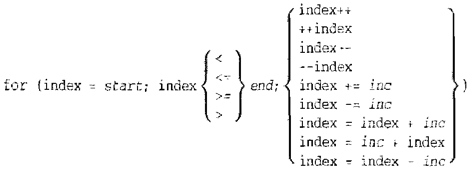
\includegraphics[width=10cm]{../imagenes/for_form.png} 
\end{center}
\caption{Para que la claúsula \texttt{for} tenga efecto sobre un ciclo, este debe tener la forma canónica. Esta figura muestra las variantes permitidas. Los indentificadores \texttt{start}, \texttt{end} e \texttt{inc} pueden ser expresiones}
\label{fig:for_form}
\end{figure}

En el ejemplo anterior,  claramente se cumple el criterio de la forma canónica en las claúsulas de control, por lo tanto no existen salidas prematuras en el loop y el codigo será completamente paralelizable.

Durante la ejecución paralela de el ciclo, el hilo maestro crea hilos adicionale. Cada hilo tiene su propio contexto de ejecución; un espacio de direcciones conteniendo todas las variables que el hilo puede acceder. El contexto de ejecución incluye variables estáticas, datos dinámicamente alojadas en el \textit{heap}, y variables en el \textit{stack} de ejecución.

El contexto de ejecución incluye su propia \textit{stack} adicional, donde el marco de ejecución para las funciones siempre se mantiene. Cualquier variable, o puede ser \textit{compartida} o puede ser \textit{privada}. Una \textit{variable compartida} tiene la misma dirección en el contexto de ejecución de cada hilo, debido a eso todos los hilos pueden ver las variables compartidas. Una \textit{variable privada} tiene dieferentes direcciones en el contexto de ejecución de cada hilo. Un hilo puede acceder a sus propias variables privadas, pero no  a las variables privadas de otro hilo.

En el caso del pragma \textit{parallel for}, por default todas las variables son compartidas, con la excepción de que la variable índice es privada.

La figura \ref{fig:var_shared_private} ilustra el acceso a variables compartidas y privadas. En este ejemplo las iteraciones del ciclo \textit{for} están siendo divididas en dos hilos. El índice \texttt{i} es una variable privada, es decir, cada hilo tiene su propia copia. Las variables \texttt{b} y \texttt{ptr}, así como los datos alojados en el \textit{heap} (parte de la memoria donde se alójan datos dinámicos, los accesos al \textit{heap} son lentos). 

\begin{figure}
\begin{center}
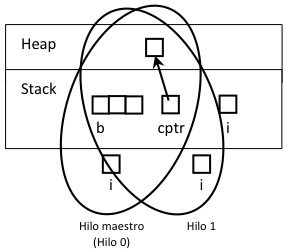
\includegraphics[width=8cm]{../imagenes/vars_share_private.png} 
\end{center}
\caption{Durante la ejecución en paralelo del ciclo, el índice \texttt{i} es una variable privada, mientras que \texttt{b}, \texttt{cptr} y los datos compartidos se encuentran en el \textit{heap}.}
\label{fig:var_shared_private}
\end{figure}

¿Cómo sabe el sistema en tiempo de ejecución cuantos hilos tiene que bifurcar un programa?. El valor de la variable de ambiente \texttt{OMP\_NUM\_THREADS} provee al sistema del número de hilos a utilizar por un programa. En Unix uno puede inspeccionar el contenido de esta variable con el comando \texttt{echo}, y para modifacar el contenido se puede usar la sintaxis \texttt{OMP\_NUM\_THREADS=n}.

Otra estrategia es modificar el número de hilos desde el código, usando las funciones necesarias para obtener los multiprocesadores disponibles por un sistema.

\section{Funci\'on \texttt{omp\_get\_num\_procs}}

La función \texttt{omp\_get\_num\_procs} regresa el número de procesadores físicos disponibles en un sistema, para ser usados por un programa paralelo, la función se define como:

\begin{lstlisting} [style=C]
int omp_get_num_procs (void)
\end{lstlisting}

El entero regresado por esta función puede ser menor que el número de procesadores físicos en un multiprocesador, dependiendo de como el sistema en tiempo de ejecución da el acceso de procesos a un procesador.

\section{Funci\'on \texttt{omp\_set\_num\_threads}}
La función \texttt{omp\_set\_num\_threads} usa un parámetro por valor para configurar el número de hilos que serán activos durante las secciones paralelas de un código

\begin{lstlisting}[style=C]
void omp_get_num_threads {int t)
\end{lstlisting}

Esta función puede ser llamada en multiples puntos del programa, así pues, se puede ajustar el nivel de paralelismo al tamaño o a las características del programa.

Configurar el número de hilos igual al número de procesadores disponibles es tan sencillo como:

\begin{lstlisting}[style=C]
int t;
....
t = omp_get_num_procs (void);
omp_get_num_threads { t );
\end{lstlisting}

\section{Declarando variables privadas}
Como segundo ejemplo usaremos el siguiente código:

\begin{lstlisting}[style=C]
for (i = 0; i < BLOCK_SIZE (id,p,n); i++) 
	for (j "' 0; j < n; j++)
		a[i][j] = MIN( a[i][j], a[i][k] + tmp[j] );
\end{lstlisting}

Si se analiza el algoritmo se ve claramente que cualquiera de los dos ciclos pueden ser claramente paralelizables. ¿Cuál se debería escoger? Si se desea paralelizar el ciclo interior (\texttt{i}), entonces el programa bifurcará  y unirá hilos por cada iteración que se realice en el ciclo externo (\texttt{j}). El \textit{overhead} (tiempo de cómputo innecesario para resolver una tarea) de bifurcar/unir puede muy bien ser mucho mayor que el tiempo ahorrado en dividir la tarea de \texttt{n} iteraciones del ciclo interior entre multiples hilos. 

Por otro lado si se paraleliza el ciclo externo, el programa solo tendrá un overhead generado por una bifurcación/unión al inicio de la primera iteración del índice \texttt{j}.

El \textbf{tamaño del grano} es el número de operaciones para realizar la comunicación de dos sistemas, es decir, la cantidad de pasos para sincronizar una tarea. En general incrementar el tamaño de grano mejora el rendimiento de un programa paralelo. Haciendo paralelo el ciclo externo resulta en un tamaño de grano mayor. Esta es la opción que se debe escoger.

Como vimos anteriormente, es sencillo decirle al compilador que ejecute en paralelo el ciclo indexado por \texttt{i}. Sin embargo, necesitamos poner atención a las variables que accede cada hilo. Por default, todas las variables son compartidas excepto el índice del ciclo (\texttt{i}). Esto facilita que los hilos se puedan comunicar, pero también puede causar ciertos problemas.

Considere que pasa, cuando multiples hilos tratan de ejecutar en paralelo, diferentes iteracionesde ciclo externo. Queremos que cada hilo trabaje através de n valores de j para cada iteración del ciclo \texttt{i}. Sin embargo, todos los hilos trataran de inicializar e incrementar la misma variable compartida j, esto implicará que no todos los hilos recorran la variable \texttt{j} para todas las \texttt{n}'s.

La solución entonces es hacer \texttt{j} una varible privada de cada hilo.

\section{Clausula \texttt{private}}

Una \textbf{claúsula}  es una componente opcional de un \texttt{pragma}. La cláusula \texttt{private} le indica al compilador que haga una o más variables privadas. La sintaxis es:

\begin{lstlisting}[style=C]
private (<lista de variables>)
\end{lstlisting}

La directiva le dice al compilador que aloje en memoria una copia de la variable para cada hilo que ejecutará el bloque \texttt{pragma} que le precede.  En este ejemplo la variable \texttt{j} sólo estará definida dentro de cada iteración del ciclo externo.

Usando la cláusula \texttt{private}, una correcta implementación en \textit{OpenMP} de ciclo doblemente anidado es:

\begin{lstlisting}[style=C]
#pragma omp parallel for private (j)
	for (i = 0; i < BLOCK_SIZE (id,p,n); i++) 
		for (j "' 0; j < n; j++)
			a[i][j] = MIN(a[i][j], a[i][k] + tmp[j]);
\end{lstlisting}

Incluso si \texttt{j} tiene asignado previamente un valor antes del ciclo paralelo interno, ninguno de los hilos podrá acceder a ese valor. Similarmente, si los hilos en tiempo de ejcución, le asignan valores a \texttt{j}, el valor de la variable compartida \texttt{j} no será afectado. En otras palabras, por default el valor de una variable privada esta indefinido cuando se bifurcan los hilos y también esta indefinido durante la unión de los mismos.

La condición de indefinición de las variables privadas durante la entrada y salida de los ciclos, reduce el tiempo de ejecución porque elimina copiados inecesarios  entre variables compartidas y sus contrapartes en variables privadas.


\section{Clausula \texttt{firstprivate}}

A veces se desea que la variable privada herede el valor de la variable compartida, considere el siguiente segmento de código:

\begin{lstlisting}[style=C]
x[0] = complex_function(); 
for (i=0; i<n; i++) {
	for(j=1; j<4;j++) 
		x[j] = g(i,x[j-1]);
	answer[i] = x[1] - x[3];
}
\end{lstlisting}

Asumiendo que la función g no tiene efectos indirectos en el código, podemos ejecutar cada iteración de ciclo externo en paralelo, siempre y cuando \texttt{x} sea una variable privada. Sin embargo, \texttt{x[0]} es inicializada ante del ciclo externo, y además, es referenciada en la primera iteración del ciclo interno. Sería impráctico mover la inicialización de \texttt{x[0]} para dentro del loop externo, porque esto consumiría tiempo de cómputo. Una mejor opción es que cada copia privada del elemento del arreglo \texttt{x[0]} herede el valor de la variable compartida que fué asignado por el hilo maestro.

Esto puede ser realizado por la cláusula \texttt{firstprivate}, la cual tiene la siguiente sintaxis:

\begin{lstlisting}[style=C]
firstprivate (<lista de variables>)
\end{lstlisting}

Esta claúsula le indica al compilador crear variables privadas que tengan valores idénticos a  los valores de las variables asignados por el hilo maestro.

Codificando en paralelo el código anterior quedaría como:

\begin{lstlisting}[style=C]
#pragma omp parallel for private (j) firstprivate(x)
x[0] = complex_function(); 
for (i=0; i<n; i++) {
	for(j=1; j<4;j++) 
		x[j] = g(i,x[j-1]);
	answer[i] = x[1] - x[3];
}
\end{lstlisting}

\section{Clausula \texttt{lastprivate}}

La cláusula \texttt{lastprivate} le indica al compilador que genere código al final del ciclo paraelo para que realize una copia de una variable privada de un hilo que tenga la última ejecución de un ciclo al hilo mestro.

Por ejemplo, supongamos que estamos paralelizando la siguiente pieza de código:

\begin{lstlisting}[style=C]
for (i=0; i<n; i++) {
	x[0] = 1.0;
	for(j=1; j<4;j++) 
		x[j] = x[j-1] * (i+1);
	sum_powers[i] = x[0] + x[1] + x[2] + x[3];
}
n_cubed = x[3]
\end{lstlisting}

En la última iteración secuencial del ciclo, \texttt{x[3]} tiene asignado el valor $n^3$.

Con el fin de tener el valor de \texttt{x[3]} fuera del ciclo paralelo, debemos declarar \texttt{x} como una variable \texttt{lastprivate}. A continuación se muestra el código paralelo correcto:

\begin{lstlisting}[style=C]
#pragma omp parallel for private (j) lastprivate(x)
for (i=0; i<n; i++) {
	x[0] = 1.0;
	for(j=1; j<4;j++) 
		x[j] = x[j-1] * (i+1);
	sum_powers[i] = x[0] + x[1] + x[2] + x[3];
}
n_cubed = x[3]
\end{lstlisting}

Un pragma \texttt{parallel for} puede contener clausulas \texttt{firstprivate} y \texttt{lasprivate}. 

\begin{lstlisting}[style=C]
#pragma omp parallel for private (j) lastprivate(x)
for (i=0; i<n; i++) {
	x[0] = 1.0;
	for(j=1; j<4;j++) 
		x[j] = x[j-1] * (i+1);
	sum_powers[i] = x[0] + x[1] + x[2] + x[3];
}
n_cubed = x[3]
\end{lstlisting}


\section{Secciones críticas}
Vamos a considerar parte de un programa en C que el valor de $\pi$ usando una forma de integración numérica llamada la regla del rectángulo.

\begin{lstlisting}[style=C]
double area,pi, x;
int i,n;
....
area = 0.0;

for (i=0; i<n; i++) {
	x = (i+0.5)/n;
	area += 4.0/(1.0 +x*x);
}
pi = area / n;
\end{lstlisting}

A diferencia de los ciclos \texttt{for} que ya hemos considerado, las iteraciones de este ciclo no son independientes. Cada iteración del ciclo lee y actualiza el valor de la variable \texttt{area}, si nosostros simplemente paralelizamos el ciclo:

\begin{lstlisting}[style=C]
double area,pi, x;
int i,n;
....
area = 0.0;

#pragma omp parallel for private (x) 
for (i=0; i<n; i++) {
	x = (i+0.5)/n;
	area += 4.0/(1.0 +x*x);   /* Condiciones de carrera */
}
pi = area / n;
\end{lstlisting}

En este código podemos finalizar sin la respuesta correcta, debido a que la sentencia de asignación a la variable \texttt{area} no es una operación atómica (indivisible), esto es llamado una condición de carrera.  Aquí vemos que él cómputo exhibe un comportamiento no determinista, es decir,  varios hilos acceden a una variable compartida (véase Figura \ref{fig:race_condition}).

Así pues, para corregir las condiciones de carrera uno debe de agregar una \textbf{sección crítica}, es decir, una porción de código que sólo un hilo puede ejecutar a la vez.


\begin{figure}
\begin{center}
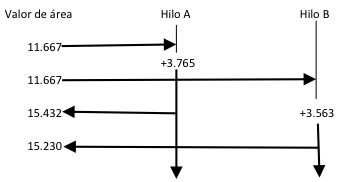
\includegraphics[width=8cm]{../imagenes/condiciones_carrera.png} 
\end{center}
\caption{Ejemplo de una condición de carrera. Cada hilo añade un valor a \texttt{area}. Sin embargo, el hilo B recupera el valor original de \texttt{area} antes que el hilo A pueda escribir un nuevo valor. Por lo tanto el valor final de \texttt{area} es incorrecto. Si el hilo B leyera el valor de \texttt{area} después de que el hilo A se actualizara, entonces el valor final de \texttt{area} sería correcto. En definitiva, la ausencia de una sección criítica puede provocar la ejecución no determinista.}
\label{fig:race_condition}
\end{figure}


\section{Pragma \texttt{critical}}

En \textit{OpenMP} se denota una sección crítica, poniendo el pragma:

\begin{lstlisting}[style=C]
#pragma omp critical
\end{lstlisting}

Al frente de bloque de código (una sola sentencia es un ejemplo trivial de un bloque de código). Este pragma le indica al compilador a forzar exclusión mutua entre los hilos que traten de ejecutar ese bloque de código.

Después de agregar el pragma \texttt{critical} al código anterior, este se ve como:

\begin{lstlisting}[style=C]
double area,pi, x;
int i,n;
....
area = 0.0;

#pragma omp parallel for private (x) 
for (i=0; i<n; i++) {
	x = (i+0.5)/n;
#pragma omp critical 
	area += 4.0/(1.0 +x*x);   /* Condiciones de carrera */
}
pi = area / n;
\end{lstlisting}

Las iteraciones del ciclo \texttt{for} son divididas entre los hilos, y sólo un hilo a la vez podrá ejecutar sentencia de asignación que actualiza la variable \texttt{area}. Sin embargo, este segmento de código exhibe una aceleración muy baja, desde que admite sólo un hilo a la vez, una sección crítica es una pieza de código secuencial dentro del ciclo \texttt{for}. El tiempo para ejecutar esta sentencia no es trivial. De aquí, que la ley de Amdahl nos dice que una sección crítica pondrá un tope muy bajo sobre la aceleración alcanzable cuando se paraleliza un ciclo \texttt{for}.

Como vemos, lo que se esta tratando de hacer es realizar una suma-reducción de \texttt{n} valores, en una sección posterior se explicará la forma adecuada de hacer esto.


\section{Reducciones}
Las reducciones son tan comunes, que \textit{OpenMP} tiene una claúsula para un pragma llamada: \texttt{parallel for}. Todo lo que se tiene que hacer es especificar la variable que guardará la reducción y la operación, y \textit{OpenMP} se encargará de los detalles, tales como guardar sumas parciales en variables privadas y poner estas en una variable global después del ciclo.

La claúsula de reducción tiene la siguiente sintaxis:

\begin{lstlisting}[style=C]
reduction (<op>:<variable>)
\end{lstlisting}

donde \texttt{<op>} es una de las operaciones de reducción mostradas en la figura x y \texttt{<variable>} es el nombre de la variable compartida que guardará el resultado de la reducción.

\begin{figure}
\begin{center}
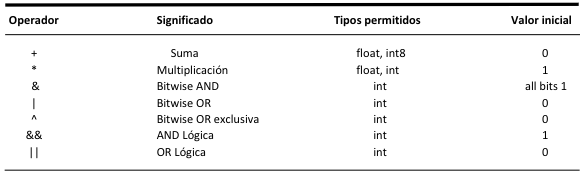
\includegraphics[width=12cm]{../imagenes/op_reduc.png} 
\end{center}
\caption{Operadores de reducción de OpenMP para C y C++}
\label{fig:op_reduc}
\end{figure}

A continuación se muestra una implementación del código que calcúla $\pi$ con la claúsula \texttt{reduction} remplazando una \texttt{critical section}.

\begin{lstlisting}[style=C]
double area,pi, x;
int i,n;
....
area = 0.0;
#pragma omp parallel for private (x)  reduction(+:area)
for (i=0; i<n; i++) {
	x = (i+0.5)/n;
	area += 4.0/(1.0 +x*x);   /* Condiciones de carrera */
}
pi = area / n;
\end{lstlisting}

En la figura \ref{fig:reduc_speed} se comparan las dos implementaciones.  Haciendo \texttt{n=100,000}. La implementación que usa la claúsula \texttt{reduction} es claramente superior,a la que usa el pragma \texttt{critical}. Esta implementación es más rápida cuando un sólo hilo está activo, y el tiempo de ejecución mejora cuando hilos adicionales son agregados.

\begin{figure}
\begin{center}
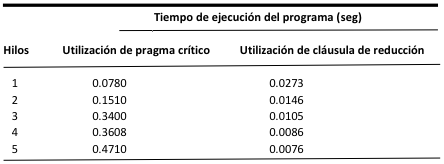
\includegraphics[width=9cm]{../imagenes/reduc_speed.png} 
\end{center}
\caption{ Tiempos de ejecución de dos programas en un Servidor Sun Enterprise 4000 que calculan $\pi$ usando la regla del rectángulo.}
\label{fig:reduc_speed}
\end{figure}


\section{Mejoras de rendimiento}
Transformar un código secuencial en un código paralelo, no es una tarea trivial e incluso, puede llegar a ser más rápida una implementación secuencial que una paralela, cuando no se respetan reglas de paralelización básicas. En secciones posteriores analizaremos como mejorar el rendimiento de programas paralelos.


\section{{Invertir ciclos}}

Considere el siguiente segmento de código:

\begin{lstlisting}[style=C]
for (i=1; i<m; i++) {
	for(j=0; j<n;j++) 
		a[i][j] = 2*a[i-1][j];
}
\end{lstlisting}

El diagrama mostrado en la figura \ref{fig:data_dependence}, ayudará a entender la dependencia de datos del código anterior. Se puede ver que dos renglones no pueden ser actualizados simultaneamente, porque hay dependencia de datos entre cada renglon. Sin embargo, las columnas pueden ser actualizadas simultaneamente.  Esto significa que el ciclo indexado por \texttt{j} puede ser ejecutado en paralelo, pero no el ciclo indexado por \texttt{i}.

Si insertamos un pragma \texttt{parallel for} antes del loop interior, el programa paralelo se ejecutará correctamente, pero no se obtendrá un buen rendimiento, debido a que no requerirá \texttt{m - 1} pasos de bifurcación/unión, es decir, un paso por cada interación del ciclo externo.

Sin embargo si se invierten los ciclos:

\begin{lstlisting}[style=C]
for(j=0; j<n;j++) 
	for (i=1; i<m; i++) 
		a[i][j] = 2*a[i-1][j];
\end{lstlisting}

\begin{figure}
\begin{center}
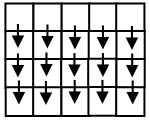
\includegraphics[width=4cm]{../imagenes/data_dependence.png} 
\end{center}
\caption{Diagrama de dependencia de datos para un determinado par de ciclos anidados donde se muestra que mientras las columnas se pueden actualizar de forma simultánea, las filas no.}
\label{fig:data_dependence}
\end{figure}

sólo un paso de bifurcación/unión es requerido (por el ciclo externo), Las dependencias de datos no han cambiado; las iteraciones del ciclo indexado por \texttt{j} siguen siendo independientes. En este sentido el código tiene la mejora necesaria, sin embargo, se debe estar conciente de como las transformaciones afectan la tasa de accesos a cache. En este caso, cada hilo esta trabajando através de las columnas de \texttt{a}. En C las matrices son guardas en orden de tipo \textit{row-mayor}, debido a esto invertir ciclos puede bajar la tasa de accesos a cache, dependiendo  de m,n, el número de hilos activos  y la arquitectura del sistema que se este usando.

\section{Ejecutar ciclos de manera condicional}
Si un ciclo no tiene suficientes iteraciones el tiempo gastado en bifurcar y unir hilos puede exceder el tiempo ahorrado por dividir las iteraciones de un ciclo entre multiples hilos. Considere, por ejemplo, la implementación paralela de la regla del rectángulo:

\begin{lstlisting}[style=C]
area = 0.0;
#pragma omp parallel for private (x)  reduction(+:area)
	for (i=0; i<n; i++) {
		x = (i+0.5)/n;
		area += 4.0/(1.0 +x*x);   /* Condiciones de carrera */
	}
	pi = area / n;
\end{lstlisting}

La figura \ref{fig:time_pi} reporta el tiempo de ejecución promedio de este programa, para varios valores de \texttt{n} y varios numeros de hilos. Como se puede ver,  cuando \texttt{n} es igual a 100, el tiempo de ejecución secuencial es demasiado pequeño, y por eso usar hilos sólo incrementará la totalidad del tiempo de ejecución. Cuando \texttt{n} es 100,000 el programa paralelo ejecutado en 4 hilos alcanza una aceleración de 3.16 sobre el programa secuencial.

\begin{figure}
\begin{center}
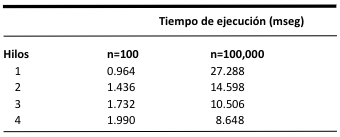
\includegraphics[width=9cm]{../imagenes/time_pi.png} 
\end{center}
\caption{Tiempo de ejecución en un servidor Sun Enterprise Server 4000 de un programa en C paralelizado que calcula $\pi$ usando la regla del rectángulo}
\label{fig:time_pi}
\end{figure}

La claúsula \texttt{if} da la habilidad de indicarle al compilador, sí un ciclo debería ser ejecutado en paralelo o secuencialmente (en tiempo de ejecución). La claúsula tiene la siguiente sintaxis:

\begin{lstlisting}[style=C]
if (<expresion escalar>)
\end{lstlisting}

Si la expresión escalar evalúa verdadero, el ciclo será ejecutado en paralelo. En otro caso se ejecutará serialmente.

Por ejemplo, a continuación se muestra como se podría añadir la claúsula \texttt{if} al código anterior y serializar el código para \texttt{n}'s menores a 5000:

\begin{lstlisting}[style=C]
area = 0.0;
#pragma omp parallel for private (x)  reduction(+:area) if (n > 5000)
	for (i=0; i<n; i++) {
	.....
\end{lstlisting}


\section{Calendarizando los ciclos}
En algunos ciclos el tiempo necesario para ejecutar iteraciones del ciclo varía considerablemente. Por ejemplo, consideremos el siguiente ciclo doblemente anidado que inicializa la triangular superior de una matríz:

\begin{lstlisting}[style=C]
for (i=0; i<n; i++)
	for ( j=i; j<n; i++)
		a[i][j] = alpha_omega(i,j);
\end{lstlisting}

Asumiendo que no hay dependencia de datos entre las iteraciones, podriamos preferir ejecutar el ciclo externo en paralelo con el fin de minimizar el \textit{overhead} de bifurcar y unir  los hilos. Si cada llamada la función \texttt{alpha\_omega} toma la misma cantidad de tiempo, entonces la primera iteración del ciclo externo (cuando \texttt{i} es igual 0) requiere \texttt{n} veces más trabajo que la última iteración (cuando \texttt{i} es igual \texttt{n-1}). Invertir los ciclos no remediará el desbalanceo.

Suponga que las \texttt{n} iteraciones están siendo ejecutadas sobre t hilos. Si cada hilo es asignado a un bloque contiguo de $\lceil n/t \rceil$ ó $\lfloor n/t \rfloor$ hilos, el ciclo paralelo será pobre en eficiencia, porque algunos hilos completarán sus iteraciones mucho más rápido que otros.

La claúsula \texttt{schedule} nos permite especificar cómo la iteraciones de un ciclo deberían ser calendarizadas, es decir, alojadas a hilos. En una calendarización \texttt{static} (estática), todas las iteraciones son a los hilos antes de que ellos ejecuten cualquier iteración del ciclo \texttt{for}. En una calendarización \texttt{dynamic} (dinámica), sólo algunas de las iteraciones son alojadas a los hilos al comienzo de la ejecución del ciclo. Los hilos que completen sus tareas son elegibles para obtener trabajo adicional. El proceso de alojamiento de hilos continúa hasta que todas las iteraciones han sido distribuidas a todos los hilos. Calendarizaciones estáticas tienen un bajo \textit{overhead} pero pueden mostrar alta carga desbalanceada de trabajo. Calendarizaciones dinámicas tienen  un alto overhead pero pueden reducir el desbalanceo de carga.

En ambas calendarizaciones, dinámicas y estáticas, los rangos contíguos de iteraciones son llamados \textbf{chunks} (pedazos). Incrementar el tamaño del chunk puede reducir el overhead, e incrementar los accesos a caché. Reducir el tamaño del chunk puede permitir balancear finalmente las cargas de trabajo.

La claúsula \texttt{schedule} tiene la siguiente sintaxis:

\begin{lstlisting}[style=C]
schedule ( <type> [, <chunk>] )
\end{lstlisting}

En otras palabras, el tipo de calendarización es requierido, el tamaño del chunk es opcional. Con estos dos parámetros es fácil describir una amplia variedad de calendarizaciones:

\begin{itemize}

\item \texttt{schedule static}: Un alojamiento de $n/t$ iteraciones contiguas de cada hilo.

\item \texttt{schedule ( static, C )}: Un alojamiento intercalado de \textit{chunks} a diferentes tareas. Cada \textit{chunk} contiene C iteraciones contiguas.

\item \texttt{schedule dynamic}: Las iteraciones son alojadas dinámicamente, una a la vez a cada hilo.

\item \texttt{schedule ( dynamic, C )}: Se realiza un alojamiento dinámico de C iteraciones a la vez para cada tarea.

\item \texttt{schedule ( guided, C )}: Es un alojamiento dinámico de interaciones a tareas usando la heurística guiada \texttt{self-scheduling}. Esta heurística comienza por alojar un tamaño largo de \textit{chunk} a cada hilo e irá decrementando el tamaño del \textit{chunk} para peticiones de hilos que terminen las tareas. El tamaño del \textit{chunk} decrementa exponencialmente a un mínimo de tamaño \texttt{C}.

\item \texttt{schedule guided}: Se usa la heurística guiada \texttt{self-scheduling} con un mínimo de \textit{chunk} igual a 1.

\item \texttt{schedule (runtime)}: El tipo de calendarización será escogido en tiempo de ejecución del programa, esto es controlado por la variable de ambiente \texttt{OMP\_SCHEDULE}. Por ejemplo en sistemas Unix se requerirá el comando:
\texttt{setenv OMP\_SCHEDULE "static,1"}

\end{itemize}

Cuando la claúsula \texttt{schedule} no es incluída en el pragma \texttt{parallel for}, la mayoría de los sistemas en tiempo de ejecución por default usan un calendarizado de tareas estático de iteraciones contiguas.

Llendo de regreso al ejemplo original, un alojamiento intercalado de las iteraciones del ciclo balaceará la carga de los hilos:

\begin{lstlisting}[style=C]
#pragma omp parallel for private(j) schedule(static,1)
for (i=0; i<n; i++)
	for ( j=i; j<n; i++)
		a[i][j] = alpha_omega(i,j);
\end{lstlisting}


\section{Paralelización general de datos}
A este punto nos hemos enfocado sobre la paralelización de simples ciclos. Porque estos son quizá, la oportunidad más común para parelilizar, particualarmente en programas que ya han sido escritos en MPI.

Sin embargo, no se deberían ignorar  otras oportunidades de concurrencia, en las siguientes secciones las trataremos.

Consideremos un algorítmo que procesa listas ligadas de tareas. En el diseño,  se asume un modelo de paso de mensajes. Cómo el modelo no  es por memoria compartida , a un sólo proceso (que será llamado manejador), se le ha dado la responsabilidad de matener la lista entera de tareas. Los otros procesos (llamados trabajadores) realizarán una tarea y una vez finalizada le enviarán un mensaje al manejador, para que les asigne un nuevo trabajo.

En contraste, el modelo de memoria compartida permitirá que cada hilo acceda a la lista de \textit{tareas por hacer}, y no se necesitará un hilo manejador.

Los siguientes segmentos de código son parte de un programa que procesa tareas guardadas en una lista ligada (véase figura \ref{fig:task_algorithm}):

\begin{lstlisting}[style=C]
int main (int argc, char argv[]){
	struct job_struct job_ptr;
	struct task_struct task_ptr;
	.....
	
	task_ptr = get_next_task(&job_ptr);
	while(!task_ptr != NULL){
		complete_task (task_ptr);
		task_ptr = get_next_task(&job_ptr);
	}
	.....
}
char get_next_task(struct job_struct job_ptr){
	struct task_struct answer;
	if(job_ptr == NULL) answer = NULL;
	else{
		answer = (job_ptr)->task;
		job_ptr = (job_ptr)->next;
	}
	return answer;
}
\end{lstlisting}

¿Cómo se podría paralelizar este algorítmo? Se requiere que cada hilo realice la misma cosa: en un ciclo tomar la siguiente tarea de la lista y completar ésta, hasta que no haya más tareas que hacer. Además, se necesita estar seguros que dos hilos no toman las misma tarea. En otras palabras, es importante ejecutar la función \texttt{get\_next\_task} atómicamente.

\begin{figure}
\begin{center}
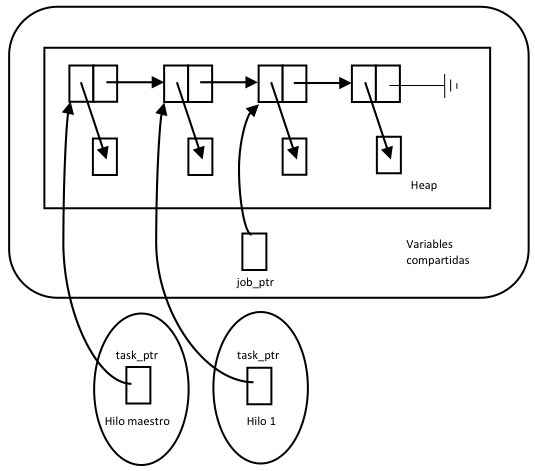
\includegraphics[width=7cm]{../imagenes/task_algorithm.png} 
\end{center}
\caption{Dos hilos realizan sus tareas a partir de una lista ligada de tareas por hacer. la variable \texttt{job\_ptr} debe ser compartida, mientras que \texttt{task\_ptr} debe ser privada.}
\label{fig:task_algorithm}
\end{figure}


\section{Pragma \texttt{parallel}}
El pragma \texttt{parallel} precede un bloque de código que debería ser ejecutado por todos los hilos, A continuación se muestra la sintaxis

\begin{lstlisting}[style=C]
#pragma omp parallel
\end{lstlisting}

Si el código es más de una sentencia, se pueden usar corchetes para definir una amplia sección de código.

Nota que a diferencia del pragma \texttt{parallel for}, el cual divide las iteraciones de un ciclo entre los hilos activos, en pragma \texttt{parallel} el bloque de código es replicado entre los hilos, sin realizar ninguna operación. Paralelizando el código anterior quedaría como:

\begin{lstlisting}[style=C]
int main (int argc, char argv[]){
	struct job_struct job_ptr;
	struct task_struct task_ptr;
	.....
#pragma omp parallel private (task_ptr)	
	task_ptr = get_next_task(&job_ptr);
	while(!task_ptr != NULL){
		complete_task (task_ptr);
		task_ptr = get_next_task(&job_ptr);
	}
	.....
}
\end{lstlisting}

Ahora se necesita estar seguro que la función \texttt{get\_next\_task} se ejecuta atómicamente. En otro caso, la ejecución puede resultar en que más de un hilo regresen de la función \texttt{get\_next\_task} con el mismo valor de \texttt{task\_ptr}.
Así que usaremos el pragma\texttt{critical} para asegurar exclusión mútua en tiempo de ejecución para el bloque que involucra la función atómica. A continuación se muestra el código:

\begin{lstlisting}[style=C]
char get_next_task(struct job_struct job_ptr){
	struct task_struct answer;
#pragma omp critical
	{
		if(job_ptr == NULL) answer = NULL;
		else{
			answer = (job_ptr)->task;
			job_ptr = (job_ptr)->next;
		}
	}
	return answer;
}
\end{lstlisting}

%%%%%%%%%%%%%%%%%%%%%
%Aqui me quede
%%%%%%%%%%%%%%%%%%%%%
\section{Función \texttt{omp\_get\_thread\_num}}
En secciones anteriores se calculó $\pi$ usando la regla del rectángulo. Ahora calcularemos $\pi$ usando el método de Monte Carlo. La idea (mostrada en la figura \ref{fig:pi_montecarlo}), es generar pares de puntos en un cuadrado unitario, es decir, donde cada coordenada varía entre 0 y 1. Posteriormente, contamos la fracción de puntos dentro del círculo, es decir, los puntos para los cuales $x^2 + y^2 \leq 1$. El valor esperado de esta fracción es $\pi / 4$; de aquí que multiplicar la fracción por 4 dará un estimado de $\pi$.

\begin{figure}
\begin{center}
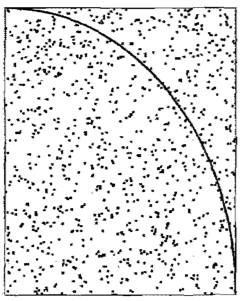
\includegraphics[width=6cm]{../imagenes/pi_montecarlo.png} 
\end{center}
\caption{ Ejemplo del algoritmo de Monte Carlo para calcular $\pi$. En este ejemplo hemos generado 1000 pares de una distribución uniforme entre 0 y 1. Hay desde 773 pares dentro del circulo, nuestra estimación de $\pi$ es 4(773/1000), o 3.092}
\label{fig:pi_montecarlo}
\end{figure}

A continuación se muestra una implementación:

\begin{lstlisting}[style=C]
int count; /*  Puntos dentro del circulo unitario */
unsigned short  xi [ 3 ] ; /*  semilla de numeros aleatorios */
int i;		
int samples;	/* puntos generados */
duble x, y ;		/* coordenadas de un punto */
samples = atoi  ( argv [ 1 ] ) ;
xi [ 0 ] =  atoi  ( argv [ 2 ] ) ;
xi [ 1 ] =  atoi  ( argv [ 3 ] ) ;
xi [ 2 ] =  atoi  ( argv [ 4 ] ) ;
count  =  0 ;
for  ( i = 0, i < samples; i++ ) {
	x = erand48 ( xi ) ;
	y = erand48 ( xi ) ;
	if  ( x * x + y * y <= 1.0 ) count++ ;
}
printf  ("pi: %7.7f\n", 4.0 * count / samples ) ;
\end{lstlisting}

Si queremos acelerar la ejecución del programa usando múltiples hilos, debemos asegurarnos de que cada hilo este generando un flujo diferente de números aleatorios. De lo contrario, cada hilo generará la misma secuencia de pares (x, y), y no habría un incremento en la precisión del programa, aunque este sea paralelizado. Por lo tanto, \texttt{xi} debe ser una variable privada, y debemos encontrar alguna manera para inicializar el arreglo de \texttt{xi} en cada hilo. Eso significa que debemos distinguir los hilos de alguna manera.

En \textit{OpenMP} cada hilo sobre un multiprocesador tiene un número de identificador único. Para obtener ese número se puede usar la función \texttt{omp\_get\_thread\_num}, la cual esta definida como:

\begin{lstlisting}[style=C]
int  omp_get_thread_num(void)
\end{lstlisting}

Si hay $t$ hilos activos, los números de identificación son números enteros que van desde $0$ a $t-1$. El hilo maestro siempre tiene el número de identificación $0$.
Asignar el número de identificación del hilo a \texttt{xi[2]} garantiza que cada hilo tenga un número de semilla aleatorio diferente.

\section{Función \texttt{omp\_get\_num\_threads}}
Con el fin de dividir las iteraciones entre los hilos, nosotros debemos conocer el número total de hilos activo. La función \texttt{omp\_get\_num\_threads}, definida como:

\begin{lstlisting}[style=C]
int  omp_get_num_threads(void)
\end{lstlisting}

regresa el número total de hilos en la región paralela. Podemos utilizar esta información, así como el número de identificación de hilo, para dividir la carga de trabajo entre los hilos disponibles.

En el siguiente ejemplo, cada hilo acumulará el conteo de puntos dentro del círculo en una variable privada. Cuando cada hilo termine el ciclo \texttt{for}, agregará su subtotal para contarlo dentro de una sección crítica.

La implementación en OpenMP se muestra a continuación

\begin{lstlisting}[style=C]
#include <stdio.h>
int main ( int argc, char *argv [] ) {
	int	  count ;	/*  Puntos dentro del circulo unitario  */
	int	  i ;
	int	 local_count ;	/* Se almacena el subtotal de hilo */
	int samples ; 	/*  Puntos generados */
	unsigned short xi ( 3 ) ;	/*  semilla de los numeros aleatorios  */
	int t ;	/*  numero total de hilos  */
	int	  tid ;	/* id del hilo */
	double	  x, y ;	/* coordenadas de un punto */

	/*  El numero de puntos y el numero de hilos son argumentos de la linea de comandos  */

	samples = atoi ( argv [ 1 ] ) ;
	omp_sat_num_threads ( atoi (argv [ 2 ]) ) ;

	count = 0 
#pragma omp parallel private ( xi, t, i, x, y, local_count )
	{
		local_count = 0 ;
		xi [ 0 ]  =  atoi ( argv [ 3 ] ) ;
		xi [ 1 ]  =  atoi ( argv [ 4 ] ) ;
		xi [ 2 ]  =  tid  = omp_get_thread_num () ;
		t  =  omp_get_num_threads () ;

		for  ( i = tid; i < samples; i += t ) {
			x = erand48 ( xi ) ;
			y = erand48 ( xi ) ;
			if ( x * x + y * y <= 1.0 )  local_count++ ;
		}
$pragma omp critical
		count  +=  local_count ;
	}
	printf ("pi : %7, %f\n" , 4.0 * count / samples ) ;
}
\end{lstlisting}


\section{Pragma \texttt{for}}

El pragma \texttt{parallel} puede ser útil también cuando se paralelizan ciclos \texttt{for}. Consideré el siguiente ciclo doblemente anidado:

\begin{lstlisting}[style=C]
#include <stdio.h>
for (i=0;i<m;i++){
	low=a[i] ;
	high=b[i] ;
	if ( low > high )	{	
		printf ( "Exiting during iteration %d\n", i ) ;
		break;
	}
	for ( j = low; j < high; j++ )
	c [ j ] = ( c [ j ] - a [ i ] / b [ j ] );
}
\end{lstlisting}

Como se observa, no se pueden ejecutar las iteraciones del ciclo externo en paralelo, ya que contiene una sentencia \texttt{break}. Si ponemos un pragma \texttt{parallel} antes del ciclo indexado por \texttt{j}, habrá un paso \textit{fork/join} por cada iteración del ciclo externo. Nos gustaría evitar este \textit{overhead}. Anteriormente, se demostró como invirtiendo los ciclos se podían solucionar este tipo de problemas, pero en este caso no funciona, debido a la dependencia de los datos.

Si ponemos el pragma \texttt{parallel} inmediatamente adelante del ciclo indexado por \texttt{i}, entonces sólo habrá un \textit{fork/join}. El comportamiento predeterminado consiste en que cada hilo ejecuta todo el código dentro del bloque. En este caso se desea que los hilos se puedan dividir las iteraciones del ciclo interno. El pragma \texttt{for} esta definido como:

\begin{lstlisting}[style=C]
#pragma omp for
\end{lstlisting}

Si se incluye el pragma \texttt{for} en el código del ejemplo anterior tenemos:

\begin{lstlisting}[style=C]
#include <stdio.h>
for (i=0;i<m;i++){
	low=a[i] ;
	high=b[i] ;
	if ( low > high )	{	
		printf ( "Exiting during iteration %d\n", i ) ;
		break;
	}
#pragma omp for
	for ( j = low; j < high; j++ )
	c [ j ] = ( c [ j ] - a [ i ] / b [ j ] );
}
\end{lstlisting}

Debido a que todos los hilos pueden acceder al \texttt{printf}, la tarea está incompleta. A continuación daremos una solución.


\section{Pragma \texttt{single}}

Hasta aquí hemos paralelizado la ejecución del ciclo indexado por \texttt{j}. Pero, ¿Qué pasa con el ciclo indexado por \texttt{i} (ciclo externo)?. El pragma \texttt{single} le indica al compilador que un sólo hilo debería de ejecutar el bloque que precede al pragma. Su sintaxis es:

\begin{lstlisting}[style=C]
#pragma omp single
\end{lstlisting}

Añadiendo el pragma \texttt{single} al ejemplo tenemos:

\begin{lstlisting}[style=C]
#include <stdio.h>
for (i=0;i<m;i++){
	low=a[i] ;
	high=b[i] ;
	if ( low > high )	{
#pragma omp single
		printf ( "Exiting during iteration %d\n", i ) ;
		break;
	}
#pragma omp for
	for ( j = low; j < high; j++ )
	c [ j ] = ( c [ j ] - a [ i ] / b [ j ] );
}
\end{lstlisting}


\section{Clúsula \texttt{nowait}}
El compilador agrega una barrera de sincronización al final de cada sentencia \texttt{prallel for}. En el ejemplo anterior hemos considerado implicitamente necesaria esta barrera. Porque estamos seguros que cada hilo ha completado una iteración del ciclo indexado por \texttt{i} antes de que cualquier otro hilo comience la siguiete itereación. De otra forma, un hilo podría cambiar el valor de \texttt{low} y \texttt{high}, alterando el numero de iteraciones realizadas por otro hilo sobre el ciclo indexado por \texttt{j}.

Por otro lado, si hacemos \texttt{low} y \texttt{high} variables privadas, no hay necesidad de la barrera al final del ciclo indexado por \texttt{j}. La claúsula \texttt{nowait}, agregada al \texttt{parallel for}, le indica al compilador que omita la barrera de sincronización al final del ciclo paralelo.

Después de hacer \texttt{high} y \texttt{low} variables privadas y sumar la claúsula \texttt{nowait}, el código del ejemplo anterior se ve como:

\begin{lstlisting}[style=C]
#include <stdio.h>
#pragma omp prallel private(i, j, low, high)
for (i=0;i<m;i++){
	low=a[i] ;
	high=b[i] ;
	if ( low > high )	{
#pragma omp single
		printf ( "Exiting during iteration %d\n", i ) ;
		break;
	}
#pragma omp for nowait
	for ( j = low; j < high; j++ )
	c [ j ] = ( c [ j ] - a [ i ] / b [ j ] );
}
\end{lstlisting}


\section{Paralelismo funcional}
Hasta este punto nos hemos enfocado en explotar el paralelismo de datos. Otra fuente de concurrencias es el pralelismo funcional. \textit{OpenMP} nos permite asignar diferentes porciones de código a diferentes hilos.

Considere, por ejemplo, el siguiente segmento de código:

\begin{lstlisting}[style=C]
v = alpha () ;
w = beta () ;
x = gamma () ;
y = delta () ;
printf ( "%6.2f\n", epsilon (x, y) ) ;
\end{lstlisting}

Si todas las funciones son libres de efectos indirectos, podemos representar las dependencias de datos, como se muestra en la figura \ref{fig:func_dependency}. Es evidente que las funciones \texttt{alfa}, \texttt{beta} y \texttt{delta} se pueden ejecutar en paralelo. Si se ejecuta estas funciones al mismo tiempo, no hay más paralelismo funcional para explotar, porque la función \texttt{gamma} depende de la ejecución de \texttt{alfa} y \texttt{beta}. Además para ejecutar \texttt{epsilon} es necesario \texttt{gamma}.

\begin{figure}
\begin{center}
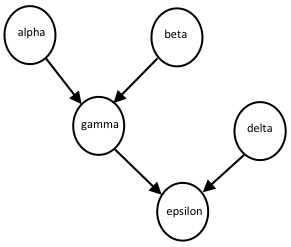
\includegraphics[width=8cm]{../imagenes/func_dependency.png} 
\end{center}
\caption{Diagrama de dependencia de datos entre varias funciones}
\label{fig:func_dependency}
\end{figure}


\section{Pragma \texttt{parallel sections}}
El pragma \texttt{parallel sections} debe preceder a un bloque de \textit{k} bloques de código que pueden ser ejecutados concurrentemente por \textit{k} hilos. Su sintaxis es:

\begin{lstlisting}[style=C]
#pragma omp parallel sections
\end{lstlisting}

\section{Pragma \texttt{section}}
El pragma \texttt{section} debe proceder a cada bloque de código que aglutine un segmento de código encerrado en un pragma \texttt{parallel sections}. (El pragma \texttt{section} puede ser omitido de dentro de la primer sección paralela desspúes del pragma \texttt{parallel sections}).

En el siguiente ejemplo consideramos que pueden ser evaluadas al mismo tiempo (concurrentemente) las llamadas a la función \texttt{alpha}, \texttt{beta}, y \texttt{delta}. En la paralelización de este segmento de código, se usa corchetes para crear un bloque de código conteniendo estos 3 sentencias de asignación. (Recuerde que una sentencia de asignación es un ejemplo trivial de un bloque de código. Por lo tanto, un bloque que contiene tres instrucciones de asignación es un bloque de tres bloques de código.)

A continuación mostramos el ejemplo:

\begin{lstlisting}[style=C]
#pragma omp parallel sections
	{
#pragma omp section	  /* pragma opcional  */
		v = alphra () ;
#pragma omp section
		w = beta () ;
#pragma omp section
		y = delta () ;
	}
	X = gamma ( v, w ) ;
	printf ( "%6.2f\n", epsilon ( x, y ) ) ;
\end{lstlisting}

Consideré que reordenamos de nuevo las declaraciones de asignación para reunir a las tres sentencias paralelas en un bloque.


\section{Pragma \texttt{sections}}

Si se revisa nuevamente la figura \ref{fig:func_dependency}, existe una segunda manera de explotar el paralelismo funcional. Como se señaló anteriormente, si ejecutamos las funciones \texttt{alpha}, \texttt{beta} y \texttt{delta} en paralelo, no hay más tareas por paralelizar. Otra manera es, ejecutar sólo las funciones \texttt{alpha} y \texttt{beta} en paralelo y posteriormente podemos ejecutar \texttt{gama} y \texttt{delta}, también en paralelo.

En este diseño tenemos dos diferentes secciones paralelas, una seguida de la otra. Además se pueden reducir costos de \textit{bifurcación/unión}, poniendo las cuatro sentencias de asignació en un sólo bloque precedido por el pragma \texttt{parallel}, y entonces se puede usar el pragma \texttt{sections} identificando el primer y segundo par de fuciones que pueden ser ejecutadas en paralelo.

El pragma \texttt{sections} tiene la siguiente sintaxis:

\begin{lstlisting}[style=C]
#pragma omp sections
\end{lstlisting}

Este pragma debe aparecer dentro de un bloque de código \texttt{paralle}. A continuación se muestra otra manera de explresar el paralelismo funcional en el segmento de código anteriormente citado:

\begin{lstlisting}[style=C]
#pragma omp parallel
{
	#pragma omp sections
	{
		#pragma omp sections		/*  Pragma opcional  */
			v = alpha () ;
		#pragma omp sections
			w = beta () ;
	}
	#pragma omp sections
	{
		#pragma omp section		/*  Pragma opcional  */
			x = gamma ( v, w ) ;
		#pragma omp section
			y = delta () ;
	}
}
printf  ("%6.2f\n", epsilon ( x, y ) ) ;
\end{lstlisting}

En un aspecto, esta solución es mejor que la primera que se prensentó, por que esta tiene dos secciones paralelas de código y cada sección cuenta con dos hilos. La primera solución tiene una única sección paralela de código que requiere tres hilos. Si sólo dos procesadores están disponibles, la segunda sección de código podría resultar con mayor eficiencia. Sea o no el caso, depende de los tiempos de ejecución de cada una de las funciones.

\section{Sumario}

\textit{OpenMP} es una API para programar usando el modelo de memoria compartida, este modelo se ejecuta como un paralelismo de \textit{bifurcación/unión}. La ejecución de un programa que usa memoria compartida, se interpreta como periodos de ejecución secuacial alternando con periodos de ejecución paralela. Un hilo maestro ejecuta el código secuencial. Cuando este alcanza un segmento paralelo, se \textit{bifurca} en otros hilos. Los hilos se comunican entre sí con variables compartidas. Al final del segmento de código paralelo, los hilos se sincronizan y se \textit{unen} en un hilo maestro.
En este trabajo, se han introducidos los \textit{pragmas} y claúsulas que pueden ser usadas para transformar un programa secuencial en C, en uno que se ejecute en paralelo sobre una arquitectura multiprocesador. Primeramente se concideró la paralelización de ciclos \texttt{for}. Para eso se utilizó, el pragma \texttt{parallel for}, que le indica al compilador que las iteraciones de ese ciclo se ejecutarán entre varios hilos. Existen ciertas restricciones entre los ciclos \texttt{for} ejecutados en paralelo. El ciclo no puede tener sentencias, \texttt{break}, \texttt{goto} o otra sentencia que permita una finalización prematura del mismo.

También se discutió como tomar ventaja del paralelismo funcional a través del uso del pragma \texttt{parallel sections}. Este pragma precede a un bloque de bloques de código, donde cada uno de los bloques interiores, o secciones, representa una tarea independiente que puede ser realizada en paralelo con otras secciones.

El pragma \texttt{parallel} precede a un bloque de código que debería ser ejecutado en paralelo en todos los hilos. Cuando todos los hilos ejecutan el mismo código, el resultado es un paralelismo muy parecido al mostrado por MPI. Un pragma \texttt{for} ó un pragma \texttt{sections} puede aparecer dentro del bloque de código marcado con un pragma \texttt{parallel}.

También se usaron pragmas que apuntan sobre áreas de código que deben ser ejecuadas secuencialmente. El pragma \texttt{critical} indica que un bloque de código forma parte de una sección crítica y la exlución mutua debe ser forzada. El pragma \texttt{single} indica que un bloque de código debe ser ejecutado secuencialmente.

Se puede añadir información adicional a un prama agregando claúsulas. La claúsula \texttt{private} indicará que cada hilo tendrá su propia copia de las variables incluidas en la claúsula. Los valores de las variables pueden ser copiados entre la variable original y las variables privadas usando las claúsulas \texttt{firstprivate} y \texttt{lastprivate}. La claúsula \texttt{reduction} le permite al compilador generar código eficiente para operaciones de reducción (suma, resta, etc...) que sucedan dentro del ciclo paralelizado. La claúsula \texttt{schedule} nos permite administrar la forma en la que las iteraciones de un ciclo son asignadas a los hilos. La claúsula \texttt{if} le permite al sistema en tiempo de ejecución si un bloque de código debe ejecutarse en paralelo ó en forrma secuencial. La claúsula \texttt{nowait} elimina la barrera de sincronización al final de un bloque paralelo.

La figura \ref{fig:pragmas_clausulas} muestra que claúsulas son validas y con que pragmas se pueden combinar.

También se examinaron varias maneras en las cuales el rendimiento de un ciclo \texttt{for} paralelo puede ser mejorado. Las estrategias son: \textit{invertir los ciclos anidados}, \textit{ciclos con paralelización condicional}, \textit{cambiar la manera en la que los hilos son calendarizados (claúsula \texttt{schecule})}.

La figura \ref{fig:comp_opemp_mpi} compara OpenMP com MPI. Ambos ambientes de programación, pueden ser usados para programar multiprocesadores. MPI es deseable para multicomputadoras. Como \textit{OpenMP} tiene variables compartidas, no es apropiado para aquitecturas que no soportan memoria compartida (multicomputadora genérica). MPI le permite al programador mayor facilidad para controlar la jerarquía de memoria. Por otro lado, \textit{OpenMP} tiene ventajas significativas que permiten hacer programas paralelizables imcrementalmente. En resúmen, a diferencia de MPI los cuales frecuentemente son muchos más largos (en líneas de código para obtener el resultado deseado) que sus contrapartes secuenciales,  los programas que usan OpenMP son susualmente prácticamente los mismo que sus pares secuenciales.

\begin{figure}
\begin{center}
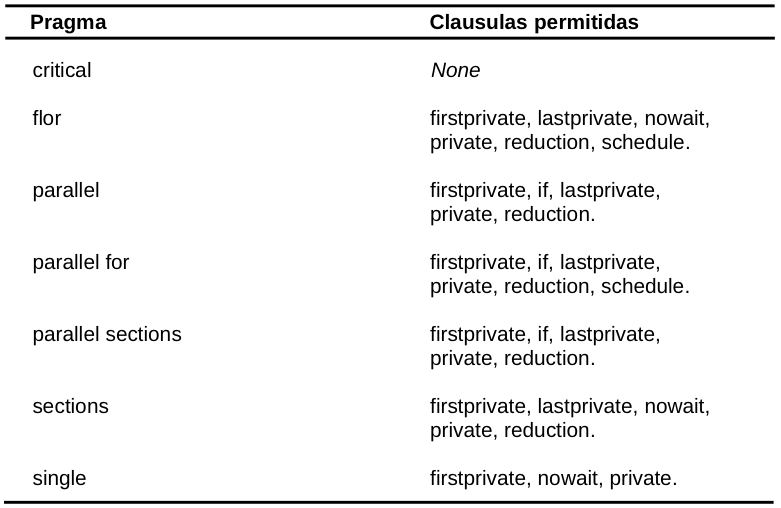
\includegraphics[width=10cm]{../imagenes/pragmas_clausulas.png} 
\end{center}
\caption{Resúmen de las clausulas que se pueden unir a un pragma (Nota: OpenMP tiene claúsulas adicionales no descritas en este trabajo)}
\label{fig:pragmas_clausulas}
\end{figure}

\begin{figure}
\begin{center}
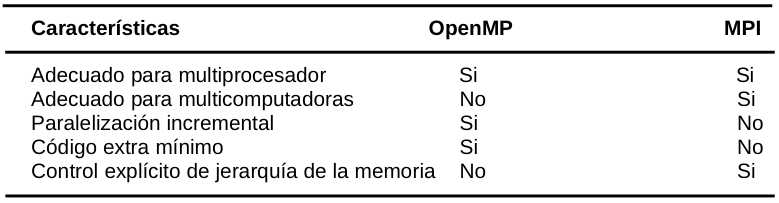
\includegraphics[width=10cm]{../imagenes/comp_opemp_mpi.png} 
\end{center}
\caption{Comparación de OpenMP y MPI}
\label{fig:comp_opemp_mpi}
\end{figure}




%%%%%#%%%%%%%%%%%%%%%%%%%%%%%%%%%%%%%%%%%%%%%%%%%%%%%%%
%\chapter{Description of the Principle}
%%\insertcode{"../Scripts/example.pl"}{Nena would be proud.} % The first argument is the script location/filename and the second is a caption for the listing
%%
%\chapter{An Example from the Later Stages}
%% your text here
%%
%\backmatter
%%
\begin{thebibliography}{99}
\bibitem{baba_books}
Books of Shrii Shrii Anandamurti (Prabhat Ranjan Sarkar): \\
http://shop.anandamarga.org/
\bibitem{anandamitra}
Avtk. Ananda Mitra Ac., \emph{The Spiritual Philosophy of Shrii Shrii Anandamurti: A Commentary on Ananda Sutram}, Ananda Marga Publications (1991) \\
ISBN: 81-7252-119-7
\end{thebibliography}
\end{document}